\documentclass[14pt]{extbook}
\usepackage{multicol, enumerate, enumitem, hyperref, color, soul, setspace, parskip, fancyhdr} %General Packages
\usepackage{amssymb, amsthm, amsmath, latexsym, units, mathtools} %Math Packages
\everymath{\displaystyle} %All math in Display Style
% Packages with additional options
\usepackage[headsep=0.5cm,headheight=12pt, left=1 in,right= 1 in,top= 1 in,bottom= 1 in]{geometry}
\usepackage[usenames,dvipsnames]{xcolor}
\usepackage{dashrule}  % Package to use the command below to create lines between items
\newcommand{\litem}[1]{\item#1\hspace*{-1cm}\rule{\textwidth}{0.4pt}}
\pagestyle{fancy}
\lhead{Progress Quiz 6}
\chead{}
\rhead{Version B}
\lfoot{1430-1829}
\cfoot{}
\rfoot{test}
\begin{document}

\begin{enumerate}
\litem{
First, find the equation of the line containing the two points below. Then, write the equation as $ y=mx+b $ and choose the intervals that contain $m$ and $b$.\[ (4, 10) \text{ and } (-4, -6) \]\begin{enumerate}[label=\Alph*.]
\item \( m \in [1, 4] \hspace*{3mm} b \in [-3, -1] \)
\item \( m \in [-5, 1] \hspace*{3mm} b \in [-18, -11] \)
\item \( m \in [1, 4] \hspace*{3mm} b \in [3, 10] \)
\item \( m \in [1, 4] \hspace*{3mm} b \in [-3, -1] \)
\item \( m \in [1, 4] \hspace*{3mm} b \in [0, 3] \)

\end{enumerate} }
\litem{
Solve the linear equation below. Then, choose the interval that contains the solution.\[ \frac{7x + 8}{2} - \frac{6x -9}{7} = \frac{7x + 8}{6} \]\begin{enumerate}[label=\Alph*.]
\item \( x \in [-6.8, -5.1] \)
\item \( x \in [-3.4, -2] \)
\item \( x \in [-1, -0.7] \)
\item \( x \in [0.6, 2.1] \)
\item \( \text{There are no real solutions.} \)

\end{enumerate} }
\litem{
First, find the equation of the line containing the two points below. Then, write the equation as $ y=mx+b $ and choose the intervals that contain $m$ and $b$.\[ (-10, 10) \text{ and } (-3, -8) \]\begin{enumerate}[label=\Alph*.]
\item \( m \in [-4.57, -1.57] \hspace*{3mm} b \in [-22.71, -10.71] \)
\item \( m \in [-4.57, -1.57] \hspace*{3mm} b \in [17, 24] \)
\item \( m \in [-4.57, -1.57] \hspace*{3mm} b \in [-6, -1] \)
\item \( m \in [-4.57, -1.57] \hspace*{3mm} b \in [13.71, 17.71] \)
\item \( m \in [1.57, 4.57] \hspace*{3mm} b \in [-1.29, 1.71] \)

\end{enumerate} }
\litem{
Write the equation of the line in the graph below in Standard form $Ax+By=C$. Then, choose the intervals that contain $A, B, \text{ and } C$.
\begin{center}
    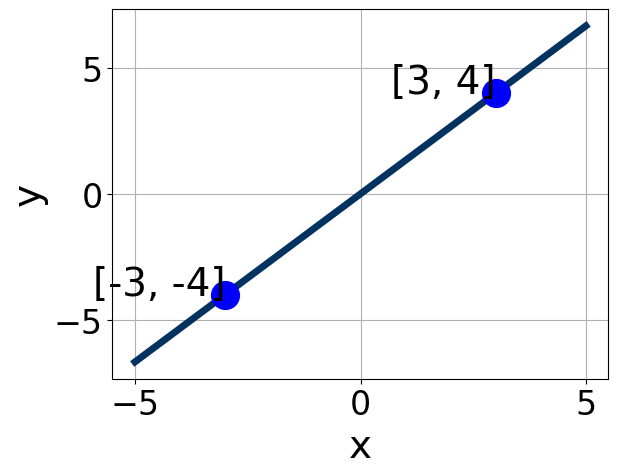
\includegraphics[width=0.5\textwidth]{../Figures/linearGraphToStandardB.png}
\end{center}
\begin{enumerate}[label=\Alph*.]
\item \( A \in [-0.1, 2.2], \hspace{3mm} B \in [-0.31, 1.03], \text{ and } \hspace{3mm} C \in [0.72, 1.47] \)
\item \( A \in [4.4, 8.4], \hspace{3mm} B \in [3.89, 4.28], \text{ and } \hspace{3mm} C \in [3.8, 5.66] \)
\item \( A \in [-0.1, 2.2], \hspace{3mm} B \in [-1.84, -0.09], \text{ and } \hspace{3mm} C \in [-2.35, -0.65] \)
\item \( A \in [4.4, 8.4], \hspace{3mm} B \in [-5.04, -3.95], \text{ and } \hspace{3mm} C \in [-4.46, -3.92] \)
\item \( A \in [-6.1, -4.8], \hspace{3mm} B \in [-5.04, -3.95], \text{ and } \hspace{3mm} C \in [-4.46, -3.92] \)

\end{enumerate} }
\litem{
Solve the equation below. Then, choose the interval that contains the solution.\[ -11(4x + 3) = -16(-5x + 7) \]\begin{enumerate}[label=\Alph*.]
\item \( x \in [0.45, 0.73] \)
\item \( x \in [-1.65, -0.85] \)
\item \( x \in [0.9, 1.17] \)
\item \( x \in [3.58, 4.2] \)
\item \( \text{There are no real solutions.} \)

\end{enumerate} }
\litem{
Solve the linear equation below. Then, choose the interval that contains the solution.\[ \frac{3x + 5}{7} - \frac{4x -5}{4} = \frac{-3x + 7}{8} \]\begin{enumerate}[label=\Alph*.]
\item \( x \in [13.27, 18.27] \)
\item \( x \in [-10.18, -6.18] \)
\item \( x \in [-3.54, 0.46] \)
\item \( x \in [3.55, 8.55] \)
\item \( \text{There are no real solutions.} \)

\end{enumerate} }
\litem{
Solve the equation below. Then, choose the interval that contains the solution.\[ -8(-7x -17) = -3(4x -6) \]\begin{enumerate}[label=\Alph*.]
\item \( x \in [-4.6, -2.7] \)
\item \( x \in [1.9, 2.5] \)
\item \( x \in [-3.2, -2.1] \)
\item \( x \in [-2.1, -0.8] \)
\item \( \text{There are no real solutions.} \)

\end{enumerate} }
\litem{
Find the equation of the line described below. Write the linear equation as $ y=mx+b $ and choose the intervals that contain $m$ and $b$.\[ \text{Parallel to } 3 x + 8 y = 3 \text{ and passing through the point } (10, -3). \]\begin{enumerate}[label=\Alph*.]
\item \( m \in [0.3, 1.6] \hspace*{3mm} b \in [-10.2, -5.8] \)
\item \( m \in [-5.1, -2.1] \hspace*{3mm} b \in [0.2, 1.2] \)
\item \( m \in [-1.7, -0.2] \hspace*{3mm} b \in [0.2, 1.2] \)
\item \( m \in [-1.7, -0.2] \hspace*{3mm} b \in [-1.4, 0.6] \)
\item \( m \in [-1.7, -0.2] \hspace*{3mm} b \in [-14, -11.7] \)

\end{enumerate} }
\litem{
Write the equation of the line in the graph below in Standard form $Ax+By=C$. Then, choose the intervals that contain $A, B, \text{ and } C$.
\begin{center}
    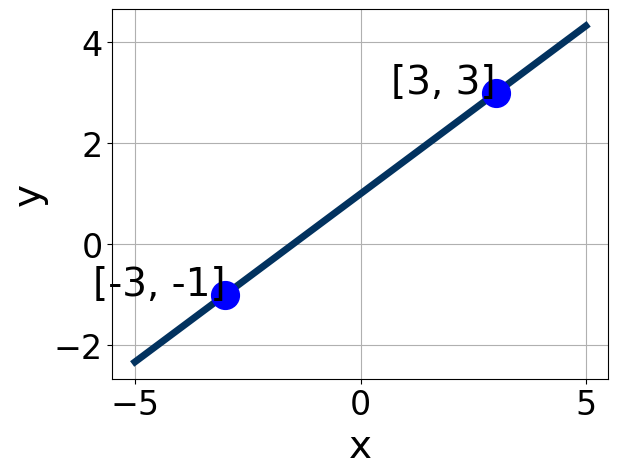
\includegraphics[width=0.5\textwidth]{../Figures/linearGraphToStandardCopyB.png}
\end{center}
\begin{enumerate}[label=\Alph*.]
\item \( A \in [0.5, 3.5], \hspace{3mm} B \in [-0.4, 1.7], \text{ and } \hspace{3mm} C \in [3.3, 6.7] \)
\item \( A \in [0.5, 3.5], \hspace{3mm} B \in [-1.59, -0.03], \text{ and } \hspace{3mm} C \in [-5.7, -2.7] \)
\item \( A \in [4, 10], \hspace{3mm} B \in [1.92, 2.42], \text{ and } \hspace{3mm} C \in [5.7, 8.1] \)
\item \( A \in [4, 10], \hspace{3mm} B \in [-2.26, -1.25], \text{ and } \hspace{3mm} C \in [-10.8, -7.8] \)
\item \( A \in [-11, -2], \hspace{3mm} B \in [-2.26, -1.25], \text{ and } \hspace{3mm} C \in [-10.8, -7.8] \)

\end{enumerate} }
\litem{
Find the equation of the line described below. Write the linear equation as $ y=mx+b $ and choose the intervals that contain $m$ and $b$.\[ \text{Parallel to } 8 x - 7 y = 6 \text{ and passing through the point } (-8, 4). \]\begin{enumerate}[label=\Alph*.]
\item \( m \in [1.13, 1.43] \hspace*{3mm} b \in [-14.14, -8.14] \)
\item \( m \in [1.13, 1.43] \hspace*{3mm} b \in [13.14, 17.14] \)
\item \( m \in [1.13, 1.43] \hspace*{3mm} b \in [8, 13] \)
\item \( m \in [-1.28, -0.88] \hspace*{3mm} b \in [-7.14, -3.14] \)
\item \( m \in [0.67, 1.1] \hspace*{3mm} b \in [13.14, 17.14] \)

\end{enumerate} }
\end{enumerate}

\end{document}